%%%%%%%%%%%%%%%%%%%%%%%%%%%%%%%%%%%%%%%%%%%%%%%%%
\section[Reconstruction]{Reconstruction}
%------------------------------------------------
%++++++++++++++++++++++++++++++++++++++++++++++++
\subsection{Modélisation théorique}
%++++++++++++++++++++++++++++++++++++++++++++++++

\begin{frame}
\frametitle{Les différents repères}

\begin{minipage}{0.48\textwidth}
    \centering
    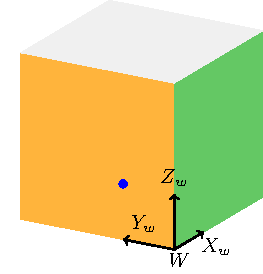
\includegraphics[width=\linewidth]{capture/cube_tikz.pdf}
    \vspace{0.5em}
    
    {\footnotesize\textbf{Représentation du cube (vue 3D)}}
\end{minipage}
\hfill
\begin{minipage}{0.48\textwidth}
    \centering
    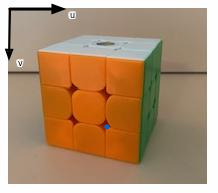
\includegraphics[width=\linewidth]{capture/cube_repere.png}
    \vspace{0.5em}

    {\footnotesize\textbf{Cube sur une image}}
\end{minipage}

\end{frame}


\begin{frame}
\frametitle{Les différents repères}

\begin{minipage}[c]{0.48\linewidth}
  \centering
  \begin{overlayarea}{0.9\linewidth}{4cm}
    \hspace*{-1cm}
    \begin{tikzpicture}[x=0.75pt,y=0.75pt,yscale=-1,xscale=1, scale=0.6]
    \only<1>{


\tikzset{every picture/.style={line width=0.75pt}} %set default line width to 0.75pt        

\begin{tikzpicture}[x=0.75pt,y=0.75pt,yscale=-1,xscale=1]
%uncomment if require: \path (0,300); %set diagram left start at 0, and has height of 300

%Shape: Rectangle [id:dp9723727103024109] 
\draw  [line width=0.75]  (273.11,2.68) -- (273.16,155.68) -- (150.53,258.66) -- (150.47,105.66) -- cycle ;
%Shape: Circle [id:dp9239162914529644] 
\draw   (170.87,132.32) .. controls (172.23,131.96) and (173.33,132.77) .. (173.33,134.13) .. controls (173.33,135.49) and (172.23,136.89) .. (170.87,137.26) .. controls (169.5,137.62) and (168.4,136.81) .. (168.4,135.45) .. controls (168.4,134.09) and (169.5,132.69) .. (170.87,132.32) -- cycle ;
%Straight Lines [id:da4507743094695521] 
\draw  [dash pattern={on 0.84pt off 2.51pt}]  (211.82,130.67) -- (45,134.7) ;
%Shape: Circle [id:dp9335082203579057] 
\draw   (499.62,131.92) .. controls (500.98,131.55) and (502.08,132.36) .. (502.08,133.72) .. controls (502.08,135.09) and (500.98,136.49) .. (499.62,136.85) .. controls (498.25,137.22) and (497.15,136.41) .. (497.15,135.05) .. controls (497.15,133.68) and (498.25,132.28) .. (499.62,131.92) -- cycle ;
%Shape: Circle [id:dp5162114026007054] 
\draw  [color={rgb, 255:red, 241; green, 53; blue, 53 }  ,draw opacity=1 ] (512.82,105.92) .. controls (514.18,105.55) and (515.28,106.36) .. (515.28,107.72) .. controls (515.28,109.09) and (514.18,110.49) .. (512.82,110.85) .. controls (511.45,111.22) and (510.35,110.41) .. (510.35,109.05) .. controls (510.35,107.68) and (511.45,106.28) .. (512.82,105.92) -- cycle ;
%Shape: Circle [id:dp4319786220460511] 
\draw  [fill={rgb, 255:red, 0; green, 0; blue, 0 }  ,fill opacity=1 ] (321.12,132.42) .. controls (322.48,132.42) and (323.58,133.52) .. (323.58,134.88) .. controls (323.58,136.25) and (322.48,137.35) .. (321.12,137.35) .. controls (319.75,137.35) and (318.65,136.25) .. (318.65,134.88) .. controls (318.65,133.52) and (319.75,132.42) .. (321.12,132.42) -- cycle ;
%Straight Lines [id:da5164589906920809] 
\draw    (321.12,134.88) -- (321.97,70.75) ;
\draw [shift={(322,68.75)}, rotate = 90.77] [color={rgb, 255:red, 0; green, 0; blue, 0 }  ][line width=0.75]    (10.93,-3.29) .. controls (6.95,-1.4) and (3.31,-0.3) .. (0,0) .. controls (3.31,0.3) and (6.95,1.4) .. (10.93,3.29)   ;
%Straight Lines [id:da7854412907443913] 
\draw    (321.12,134.88) -- (253.5,134.75) ;
\draw [shift={(251.5,134.75)}, rotate = 0.11] [color={rgb, 255:red, 0; green, 0; blue, 0 }  ][line width=0.75]    (10.93,-3.29) .. controls (6.95,-1.4) and (3.31,-0.3) .. (0,0) .. controls (3.31,0.3) and (6.95,1.4) .. (10.93,3.29)   ;
%Straight Lines [id:da3058610918194634] 
\draw    (321.12,134.88) -- (272.48,176.16) ;
\draw [shift={(270.95,177.45)}, rotate = 319.68] [color={rgb, 255:red, 0; green, 0; blue, 0 }  ][line width=0.75]    (10.93,-3.29) .. controls (6.95,-1.4) and (3.31,-0.3) .. (0,0) .. controls (3.31,0.3) and (6.95,1.4) .. (10.93,3.29)   ;
%Straight Lines [id:da5453100201962917] 
\draw  [dash pattern={on 4.5pt off 4.5pt}]  (149.63,172.62) -- (150.47,105.66) ;
\draw [shift={(149.61,174.62)}, rotate = 270.72] [color={rgb, 255:red, 0; green, 0; blue, 0 }  ][line width=0.75]    (10.93,-3.29) .. controls (6.95,-1.4) and (3.31,-0.3) .. (0,0) .. controls (3.31,0.3) and (6.95,1.4) .. (10.93,3.29)   ;
%Straight Lines [id:da4691798453437107] 
\draw  [dash pattern={on 4.5pt off 4.5pt}]  (199.11,64.39) -- (150.47,105.66) ;
\draw [shift={(200.64,63.1)}, rotate = 139.68] [color={rgb, 255:red, 0; green, 0; blue, 0 }  ][line width=0.75]    (10.93,-3.29) .. controls (6.95,-1.4) and (3.31,-0.3) .. (0,0) .. controls (3.31,0.3) and (6.95,1.4) .. (10.93,3.29)   ;
%Straight Lines [id:da9224741393814412] 
\draw [color={rgb, 255:red, 241; green, 45; blue, 45 }  ,draw opacity=1 ]   (512.82,108.38) -- (192.48,152.97) ;
\draw [shift={(190.5,153.25)}, rotate = 352.08] [color={rgb, 255:red, 241; green, 45; blue, 45 }  ,draw opacity=1 ][line width=0.75]    (10.93,-3.29) .. controls (6.95,-1.4) and (3.31,-0.3) .. (0,0) .. controls (3.31,0.3) and (6.95,1.4) .. (10.93,3.29)   ;
%Shape: Circle [id:dp7585208638434278] 
\draw  [color={rgb, 255:red, 241; green, 53; blue, 53 }  ,draw opacity=1 ] (190.5,150.78) .. controls (191.86,150.42) and (192.97,151.23) .. (192.97,152.59) .. controls (192.97,153.95) and (191.86,155.35) .. (190.5,155.72) .. controls (189.14,156.08) and (188.03,155.27) .. (188.03,153.91) .. controls (188.03,152.55) and (189.14,151.15) .. (190.5,150.78) -- cycle ;
%Shape: Cube [id:dp7714367112041981] 
\draw   (499.62,131.92) -- (520.32,111.22) -- (568.62,111.22) -- (568.62,160.52) -- (547.92,181.22) -- (499.62,181.22) -- cycle ; \draw   (568.62,111.22) -- (547.92,131.92) -- (499.62,131.92) ; \draw   (547.92,131.92) -- (547.92,181.22) ;

% Text Node
\draw (517,97.9) node [anchor=north west][inner sep=0.75pt]  [font=\footnotesize,color={rgb, 255:red, 167; green, 17; blue, 17 }  ,opacity=1 ]  {$P$};
% Text Node
\draw (324,59.9) node [anchor=north west][inner sep=0.75pt]  [font=\footnotesize]  {$\vec{j}$};
% Text Node
\draw (280.5,178.9) node [anchor=north west][inner sep=0.75pt]  [font=\footnotesize]  {$\vec{i}$};
% Text Node
\draw (324.43,139.84) node [anchor=north west][inner sep=0.75pt]  [font=\footnotesize]  {$O$};
% Text Node
\draw (252,112.9) node [anchor=north west][inner sep=0.75pt]  [font=\footnotesize]  {$\vec{k}$};
% Text Node
\draw (158.65,118.28) node [anchor=north west][inner sep=0.75pt]  [font=\footnotesize]  {$C$};
% Text Node
\draw (156,62.9) node [anchor=north west][inner sep=0.75pt]  [font=\footnotesize]  {$\vec{u}$};
% Text Node
\draw (125.5,114.4) node [anchor=north west][inner sep=0.75pt]  [font=\footnotesize]  {$\vec{v}$};
% Text Node
\draw (184.5,155.9) node [anchor=north west][inner sep=0.75pt]  [font=\footnotesize,color={rgb, 255:red, 159; green, 16; blue, 16 }  ,opacity=1 ]  {$P'$};


\end{tikzpicture}}
    \only<2>{
%Shape: Rectangle [id:dp4318964674614302] 
\draw  [line width=0.75]  (261.98,12.03) -- (262.02,142.84) -- (150.52,236.47) -- (150.47,105.66) -- cycle ;
%Shape: Circle [id:dp8619322586517022] 
\draw  [color={rgb, 255:red, 16; green, 18; blue, 125 }  ,draw opacity=1 ][fill={rgb, 255:red, 16; green, 18; blue, 125 }  ,fill opacity=1 ] (350.47,93.07) .. controls (351.83,92.71) and (352.93,93.52) .. (352.93,94.88) .. controls (352.93,96.24) and (351.83,97.64) .. (350.47,98.01) .. controls (349.1,98.37) and (348,97.56) .. (348,96.2) .. controls (348,94.84) and (349.1,93.44) .. (350.47,93.07) -- cycle ;
%Shape: Cube [id:dp5712797611314612] 
\draw   (325.13,88.8) -- (342.27,71.67) -- (382.25,71.67) -- (382.25,112.75) -- (365.12,129.88) -- (325.13,129.88) -- cycle ; \draw   (382.25,71.67) -- (365.12,88.8) -- (325.13,88.8) ; \draw   (365.12,88.8) -- (365.12,129.88) ;
%Shape: Rectangle [id:dp6697517945708218] 
\draw  [color={rgb, 255:red, 255; green, 255; blue, 255 }  ,draw opacity=1 ] (41.02,5.34) -- (469,5.34) -- (469,280.34) -- (41.02,280.34) -- cycle ;

% Text Node
\draw (358,50.9) node [anchor=north west][inner sep=0.75pt]  [font=\footnotesize,color={rgb, 255:red, 16; green, 18; blue, 125 }  ,opacity=1 ]  {$M$};}
    \only<3>{
%Shape: Rectangle [id:dp028088791950111824] 
\draw  [line width=0.75]  (261.98,12.03) -- (262.02,142.84) -- (150.52,236.47) -- (150.47,105.66) -- cycle ;
%Shape: Circle [id:dp7031182719098343] 
\draw  [color={rgb, 255:red, 16; green, 18; blue, 125 }  ,draw opacity=1 ][fill={rgb, 255:red, 16; green, 18; blue, 125 }  ,fill opacity=1 ] (350.47,93.07) .. controls (351.83,92.71) and (352.93,93.52) .. (352.93,94.88) .. controls (352.93,96.24) and (351.83,97.64) .. (350.47,98.01) .. controls (349.1,98.37) and (348,97.56) .. (348,96.2) .. controls (348,94.84) and (349.1,93.44) .. (350.47,93.07) -- cycle ;
%Shape: Circle [id:dp5293499977985842] 
\draw  [fill={rgb, 255:red, 0; green, 0; blue, 0 }  ,fill opacity=1 ] (365.12,130.42) .. controls (366.48,130.42) and (367.58,131.52) .. (367.58,132.88) .. controls (367.58,134.25) and (366.48,135.35) .. (365.12,135.35) .. controls (363.75,135.35) and (362.65,134.25) .. (362.65,132.88) .. controls (362.65,131.52) and (363.75,130.42) .. (365.12,130.42) -- cycle ;
%Straight Lines [id:da017082435473012803] 
\draw    (365.12,130.42) -- (331,129.27) ;
\draw [shift={(329,129.2)}, rotate = 1.93] [color={rgb, 255:red, 0; green, 0; blue, 0 }  ][line width=0.75]    (10.93,-3.29) .. controls (6.95,-1.4) and (3.31,-0.3) .. (0,0) .. controls (3.31,0.3) and (6.95,1.4) .. (10.93,3.29)   ;
%Straight Lines [id:da5599496973424118] 
\draw    (365.12,130.42) -- (380.86,114.19) ;
\draw [shift={(382.25,112.75)}, rotate = 134.12] [color={rgb, 255:red, 0; green, 0; blue, 0 }  ][line width=0.75]    (10.93,-3.29) .. controls (6.95,-1.4) and (3.31,-0.3) .. (0,0) .. controls (3.31,0.3) and (6.95,1.4) .. (10.93,3.29)   ;
%Straight Lines [id:da6797087519996778] 
\draw    (364.65,132.88) -- (364.04,100.2) ;
\draw [shift={(364,98.2)}, rotate = 88.93] [color={rgb, 255:red, 0; green, 0; blue, 0 }  ][line width=0.75]    (10.93,-3.29) .. controls (6.95,-1.4) and (3.31,-0.3) .. (0,0) .. controls (3.31,0.3) and (6.95,1.4) .. (10.93,3.29)   ;
%Shape: Cube [id:dp7302403803638008] 
\draw   (325.13,88.8) -- (342.27,71.67) -- (382.25,71.67) -- (382.25,112.75) -- (365.12,129.88) -- (325.13,129.88) -- cycle ; \draw   (382.25,71.67) -- (365.12,88.8) -- (325.13,88.8) ; \draw   (365.12,88.8) -- (365.12,129.88) ;
%Shape: Rectangle [id:dp8228992922802219] 
\draw  [color={rgb, 255:red, 255; green, 255; blue, 255 }  ,draw opacity=1 ] (41.02,5.34) -- (469,5.34) -- (469,280.34) -- (41.02,280.34) -- cycle ;

% Text Node
\draw (358,50.9) node [anchor=north west][inner sep=0.75pt]  [font=\footnotesize,color={rgb, 255:red, 16; green, 18; blue, 125 }  ,opacity=1 ]  {$M$};
% Text Node
\draw (364.65,136.28) node [anchor=north west][inner sep=0.75pt]  [font=\footnotesize]  {$W$};

}
    \only<4>{
%Shape: Rectangle [id:dp10737819772185131] 
\draw  [line width=0.75]  (261.98,12.03) -- (262.02,142.84) -- (150.52,236.47) -- (150.47,105.66) -- cycle ;
%Shape: Circle [id:dp372963627496946] 
\draw  [color={rgb, 255:red, 16; green, 18; blue, 125 }  ,draw opacity=1 ][fill={rgb, 255:red, 16; green, 18; blue, 125 }  ,fill opacity=1 ] (350.47,93.07) .. controls (351.83,92.71) and (352.93,93.52) .. (352.93,94.88) .. controls (352.93,96.24) and (351.83,97.64) .. (350.47,98.01) .. controls (349.1,98.37) and (348,97.56) .. (348,96.2) .. controls (348,94.84) and (349.1,93.44) .. (350.47,93.07) -- cycle ;
%Shape: Circle [id:dp4055144555634762] 
\draw  [fill={rgb, 255:red, 0; green, 0; blue, 0 }  ,fill opacity=1 ] (365.12,130.42) .. controls (366.48,130.42) and (367.58,131.52) .. (367.58,132.88) .. controls (367.58,134.25) and (366.48,135.35) .. (365.12,135.35) .. controls (363.75,135.35) and (362.65,134.25) .. (362.65,132.88) .. controls (362.65,131.52) and (363.75,130.42) .. (365.12,130.42) -- cycle ;
%Straight Lines [id:da033990839101548764] 
\draw  [dash pattern={on 4.5pt off 4.5pt}]  (150.02,143.52) -- (150.47,105.66) ;
\draw [shift={(150,145.52)}, rotate = 270.68] [color={rgb, 255:red, 0; green, 0; blue, 0 }  ][line width=0.75]    (10.93,-3.29) .. controls (6.95,-1.4) and (3.31,-0.3) .. (0,0) .. controls (3.31,0.3) and (6.95,1.4) .. (10.93,3.29)   ;
%Straight Lines [id:da45416316832348713] 
\draw  [dash pattern={on 4.5pt off 4.5pt}]  (182.47,78.8) -- (150.47,105.66) ;
\draw [shift={(184,77.52)}, rotate = 139.99] [color={rgb, 255:red, 0; green, 0; blue, 0 }  ][line width=0.75]    (10.93,-3.29) .. controls (6.95,-1.4) and (3.31,-0.3) .. (0,0) .. controls (3.31,0.3) and (6.95,1.4) .. (10.93,3.29)   ;
%Straight Lines [id:da2556447217923111] 
\draw    (365.12,130.42) -- (331,129.27) ;
\draw [shift={(329,129.2)}, rotate = 1.93] [color={rgb, 255:red, 0; green, 0; blue, 0 }  ][line width=0.75]    (10.93,-3.29) .. controls (6.95,-1.4) and (3.31,-0.3) .. (0,0) .. controls (3.31,0.3) and (6.95,1.4) .. (10.93,3.29)   ;
%Straight Lines [id:da09787654361591336] 
\draw    (365.12,130.42) -- (380.86,114.19) ;
\draw [shift={(382.25,112.75)}, rotate = 134.12] [color={rgb, 255:red, 0; green, 0; blue, 0 }  ][line width=0.75]    (10.93,-3.29) .. controls (6.95,-1.4) and (3.31,-0.3) .. (0,0) .. controls (3.31,0.3) and (6.95,1.4) .. (10.93,3.29)   ;
%Straight Lines [id:da23688764512738059] 
\draw    (364.65,132.88) -- (364.04,100.2) ;
\draw [shift={(364,98.2)}, rotate = 88.93] [color={rgb, 255:red, 0; green, 0; blue, 0 }  ][line width=0.75]    (10.93,-3.29) .. controls (6.95,-1.4) and (3.31,-0.3) .. (0,0) .. controls (3.31,0.3) and (6.95,1.4) .. (10.93,3.29)   ;
%Shape: Cube [id:dp10483038398606548] 
\draw   (325.13,88.8) -- (342.27,71.67) -- (382.25,71.67) -- (382.25,112.75) -- (365.12,129.88) -- (325.13,129.88) -- cycle ; \draw   (382.25,71.67) -- (365.12,88.8) -- (325.13,88.8) ; \draw   (365.12,88.8) -- (365.12,129.88) ;
%Shape: Rectangle [id:dp9630082762596079] 
\draw  [color={rgb, 255:red, 255; green, 255; blue, 255 }  ,draw opacity=1 ] (41.02,5.34) -- (469,5.34) -- (469,280.34) -- (41.02,280.34) -- cycle ;

% Text Node
\draw (358,50.9) node [anchor=north west][inner sep=0.75pt]  [font=\footnotesize,color={rgb, 255:red, 16; green, 18; blue, 125 }  ,opacity=1 ]  {$M$};
% Text Node
\draw (364.65,136.28) node [anchor=north west][inner sep=0.75pt]  [font=\footnotesize]  {$W$};
% Text Node
\draw (154,71.9) node [anchor=north west][inner sep=0.75pt]  [font=\footnotesize]  {$u'$};
% Text Node
\draw (129.5,109.4) node [anchor=north west][inner sep=0.75pt]  [font=\footnotesize]  {$v'$};}
    \only<5>{
\draw  [line width=0.75]  (261.98,12.03) -- (262.02,142.84) -- (150.52,236.47) -- (150.47,105.66) -- cycle ;
%Shape: Circle [id:dp0391503239902703] 
\draw  [color={rgb, 255:red, 16; green, 18; blue, 125 }  ,draw opacity=1 ][fill={rgb, 255:red, 16; green, 18; blue, 125 }  ,fill opacity=1 ] (350.47,93.07) .. controls (351.83,92.71) and (352.93,93.52) .. (352.93,94.88) .. controls (352.93,96.24) and (351.83,97.64) .. (350.47,98.01) .. controls (349.1,98.37) and (348,97.56) .. (348,96.2) .. controls (348,94.84) and (349.1,93.44) .. (350.47,93.07) -- cycle ;
%Shape: Circle [id:dp8654606077158083] 
\draw  [fill={rgb, 255:red, 0; green, 0; blue, 0 }  ,fill opacity=1 ] (365.12,130.42) .. controls (366.48,130.42) and (367.58,131.52) .. (367.58,132.88) .. controls (367.58,134.25) and (366.48,135.35) .. (365.12,135.35) .. controls (363.75,135.35) and (362.65,134.25) .. (362.65,132.88) .. controls (362.65,131.52) and (363.75,130.42) .. (365.12,130.42) -- cycle ;
%Straight Lines [id:da3675337375445349] 
\draw  [dash pattern={on 4.5pt off 4.5pt}]  (150.02,143.52) -- (150.47,105.66) ;
\draw [shift={(150,145.52)}, rotate = 270.68] [color={rgb, 255:red, 0; green, 0; blue, 0 }  ][line width=0.75]    (10.93,-3.29) .. controls (6.95,-1.4) and (3.31,-0.3) .. (0,0) .. controls (3.31,0.3) and (6.95,1.4) .. (10.93,3.29)   ;
%Straight Lines [id:da2135082456633841] 
\draw  [dash pattern={on 4.5pt off 4.5pt}]  (182.47,78.8) -- (150.47,105.66) ;
\draw [shift={(184,77.52)}, rotate = 139.99] [color={rgb, 255:red, 0; green, 0; blue, 0 }  ][line width=0.75]    (10.93,-3.29) .. controls (6.95,-1.4) and (3.31,-0.3) .. (0,0) .. controls (3.31,0.3) and (6.95,1.4) .. (10.93,3.29)   ;
%Shape: Circle [id:dp3919067214179274] 
\draw  [color={rgb, 255:red, 16; green, 18; blue, 125 }  ,draw opacity=1 ] (209.53,118.71) .. controls (210.9,118.35) and (212,119.15) .. (212,120.52) .. controls (212,121.88) and (210.9,123.28) .. (209.53,123.64) .. controls (208.17,124.01) and (207.07,123.2) .. (207.07,121.84) .. controls (207.07,120.48) and (208.17,119.08) .. (209.53,118.71) -- cycle ;
%Straight Lines [id:da13961882146045834] 
\draw [color={rgb, 255:red, 16; green, 18; blue, 125 }  ,draw opacity=1 ][fill={rgb, 255:red, 16; green, 18; blue, 125 }  ,fill opacity=1 ]   (350.47,95.54) -- (212,120.52) ;
%Straight Lines [id:da6009765896576962] 
\draw    (365.12,130.42) -- (331,129.27) ;
\draw [shift={(329,129.2)}, rotate = 1.93] [color={rgb, 255:red, 0; green, 0; blue, 0 }  ][line width=0.75]    (10.93,-3.29) .. controls (6.95,-1.4) and (3.31,-0.3) .. (0,0) .. controls (3.31,0.3) and (6.95,1.4) .. (10.93,3.29)   ;
%Straight Lines [id:da13460515919081129] 
\draw    (365.12,130.42) -- (380.86,114.19) ;
\draw [shift={(382.25,112.75)}, rotate = 134.12] [color={rgb, 255:red, 0; green, 0; blue, 0 }  ][line width=0.75]    (10.93,-3.29) .. controls (6.95,-1.4) and (3.31,-0.3) .. (0,0) .. controls (3.31,0.3) and (6.95,1.4) .. (10.93,3.29)   ;
%Straight Lines [id:da5115010168409273] 
\draw    (364.65,132.88) -- (364.04,100.2) ;
\draw [shift={(364,98.2)}, rotate = 88.93] [color={rgb, 255:red, 0; green, 0; blue, 0 }  ][line width=0.75]    (10.93,-3.29) .. controls (6.95,-1.4) and (3.31,-0.3) .. (0,0) .. controls (3.31,0.3) and (6.95,1.4) .. (10.93,3.29)   ;
%Shape: Cube [id:dp47417096557677685] 
\draw   (325.13,88.8) -- (342.27,71.67) -- (382.25,71.67) -- (382.25,112.75) -- (365.12,129.88) -- (325.13,129.88) -- cycle ; \draw   (382.25,71.67) -- (365.12,88.8) -- (325.13,88.8) ; \draw   (365.12,88.8) -- (365.12,129.88) ;
%Shape: Rectangle [id:dp12317704811349806] 
\draw  [color={rgb, 255:red, 255; green, 255; blue, 255 }  ,draw opacity=1 ] (41.02,5.34) -- (469,5.34) -- (469,280.34) -- (41.02,280.34) -- cycle ;

% Text Node
\draw (358,50.9) node [anchor=north west][inner sep=0.75pt]  [font=\footnotesize,color={rgb, 255:red, 16; green, 18; blue, 125 }  ,opacity=1 ]  {$M$};
% Text Node
\draw (364.65,136.28) node [anchor=north west][inner sep=0.75pt]  [font=\footnotesize]  {$W$};
% Text Node
\draw (154,71.9) node [anchor=north west][inner sep=0.75pt]  [font=\footnotesize]  {$u'$};
% Text Node
\draw (129.5,109.4) node [anchor=north west][inner sep=0.75pt]  [font=\footnotesize]  {$v'$};
% Text Node
\draw (210,99.9) node [anchor=north west][inner sep=0.75pt]  [font=\footnotesize,color={rgb, 255:red, 167; green, 17; blue, 17 }  ,opacity=1 ]  {$\textcolor[rgb]{0.06,0.07,0.49}{m}$};
}
    \only<6>{
%Shape: Rectangle [id:dp22091086801975413] 
\draw  [line width=0.75]  (261.98,12.03) -- (262.02,142.84) -- (150.52,236.47) -- (150.47,105.66) -- cycle ;
%Shape: Circle [id:dp3960031807548443] 
\draw  [color={rgb, 255:red, 16; green, 18; blue, 125 }  ,draw opacity=1 ][fill={rgb, 255:red, 16; green, 18; blue, 125 }  ,fill opacity=1 ] (350.47,93.07) .. controls (351.83,92.71) and (352.93,93.52) .. (352.93,94.88) .. controls (352.93,96.24) and (351.83,97.64) .. (350.47,98.01) .. controls (349.1,98.37) and (348,97.56) .. (348,96.2) .. controls (348,94.84) and (349.1,93.44) .. (350.47,93.07) -- cycle ;
%Shape: Circle [id:dp7170017338469822] 
\draw  [fill={rgb, 255:red, 0; green, 0; blue, 0 }  ,fill opacity=1 ] (365.12,130.42) .. controls (366.48,130.42) and (367.58,131.52) .. (367.58,132.88) .. controls (367.58,134.25) and (366.48,135.35) .. (365.12,135.35) .. controls (363.75,135.35) and (362.65,134.25) .. (362.65,132.88) .. controls (362.65,131.52) and (363.75,130.42) .. (365.12,130.42) -- cycle ;
%Straight Lines [id:da925005109202037] 
\draw  [dash pattern={on 4.5pt off 4.5pt}]  (150.02,143.52) -- (150.47,105.66) ;
\draw [shift={(150,145.52)}, rotate = 270.68] [color={rgb, 255:red, 0; green, 0; blue, 0 }  ][line width=0.75]    (10.93,-3.29) .. controls (6.95,-1.4) and (3.31,-0.3) .. (0,0) .. controls (3.31,0.3) and (6.95,1.4) .. (10.93,3.29)   ;
%Straight Lines [id:da7341104591578826] 
\draw  [dash pattern={on 4.5pt off 4.5pt}]  (182.47,78.8) -- (150.47,105.66) ;
\draw [shift={(184,77.52)}, rotate = 139.99] [color={rgb, 255:red, 0; green, 0; blue, 0 }  ][line width=0.75]    (10.93,-3.29) .. controls (6.95,-1.4) and (3.31,-0.3) .. (0,0) .. controls (3.31,0.3) and (6.95,1.4) .. (10.93,3.29)   ;
%Shape: Circle [id:dp054443755291766927] 
\draw  [color={rgb, 255:red, 16; green, 18; blue, 125 }  ,draw opacity=1 ] (209.53,118.71) .. controls (210.9,118.35) and (212,119.15) .. (212,120.52) .. controls (212,121.88) and (210.9,123.28) .. (209.53,123.64) .. controls (208.17,124.01) and (207.07,123.2) .. (207.07,121.84) .. controls (207.07,120.48) and (208.17,119.08) .. (209.53,118.71) -- cycle ;
%Straight Lines [id:da5500031803707174] 
\draw [color={rgb, 255:red, 16; green, 18; blue, 125 }  ,draw opacity=1 ][fill={rgb, 255:red, 16; green, 18; blue, 125 }  ,fill opacity=1 ]   (350.47,95.54) -- (212,120.52) ;
%Straight Lines [id:da19418058541638872] 
\draw    (365.12,130.42) -- (331,129.27) ;
\draw [shift={(329,129.2)}, rotate = 1.93] [color={rgb, 255:red, 0; green, 0; blue, 0 }  ][line width=0.75]    (10.93,-3.29) .. controls (6.95,-1.4) and (3.31,-0.3) .. (0,0) .. controls (3.31,0.3) and (6.95,1.4) .. (10.93,3.29)   ;
%Straight Lines [id:da06456179839803622] 
\draw    (365.12,130.42) -- (380.86,114.19) ;
\draw [shift={(382.25,112.75)}, rotate = 134.12] [color={rgb, 255:red, 0; green, 0; blue, 0 }  ][line width=0.75]    (10.93,-3.29) .. controls (6.95,-1.4) and (3.31,-0.3) .. (0,0) .. controls (3.31,0.3) and (6.95,1.4) .. (10.93,3.29)   ;
%Straight Lines [id:da6878817592231475] 
\draw    (364.65,132.88) -- (364.04,100.2) ;
\draw [shift={(364,98.2)}, rotate = 88.93] [color={rgb, 255:red, 0; green, 0; blue, 0 }  ][line width=0.75]    (10.93,-3.29) .. controls (6.95,-1.4) and (3.31,-0.3) .. (0,0) .. controls (3.31,0.3) and (6.95,1.4) .. (10.93,3.29)   ;
%Shape: Cube [id:dp39297068054343187] 
\draw   (325.13,88.8) -- (342.27,71.67) -- (382.25,71.67) -- (382.25,112.75) -- (365.12,129.88) -- (325.13,129.88) -- cycle ; \draw   (382.25,71.67) -- (365.12,88.8) -- (325.13,88.8) ; \draw   (365.12,88.8) -- (365.12,129.88) ;
%Straight Lines [id:da3701505179737167] 
\draw [color={rgb, 255:red, 0; green, 0; blue, 0 }  ,draw opacity=1 ]   (75.12,154.88) -- (75.97,90.75) ;
\draw [shift={(76,88.75)}, rotate = 90.77] [color={rgb, 255:red, 0; green, 0; blue, 0 }  ,draw opacity=1 ][line width=0.75]    (10.93,-3.29) .. controls (6.95,-1.4) and (3.31,-0.3) .. (0,0) .. controls (3.31,0.3) and (6.95,1.4) .. (10.93,3.29)   ;
%Straight Lines [id:da9863793705895071] 
\draw [color={rgb, 255:red, 0; green, 0; blue, 0 }  ,draw opacity=1 ]   (75.12,154.88) -- (116.31,128.59) ;
\draw [shift={(118,127.52)}, rotate = 147.45] [color={rgb, 255:red, 0; green, 0; blue, 0 }  ,draw opacity=1 ][line width=0.75]    (10.93,-3.29) .. controls (6.95,-1.4) and (3.31,-0.3) .. (0,0) .. controls (3.31,0.3) and (6.95,1.4) .. (10.93,3.29)   ;
%Straight Lines [id:da21691112687890424] 
\draw [color={rgb, 255:red, 0; green, 0; blue, 0 }  ,draw opacity=1 ]   (75.12,154.88) -- (128,153.57) ;
\draw [shift={(130,153.52)}, rotate = 178.57] [color={rgb, 255:red, 0; green, 0; blue, 0 }  ,draw opacity=1 ][line width=0.75]    (10.93,-3.29) .. controls (6.95,-1.4) and (3.31,-0.3) .. (0,0) .. controls (3.31,0.3) and (6.95,1.4) .. (10.93,3.29)   ;
%Straight Lines [id:da5973484313893659] 
\draw [color={rgb, 255:red, 16; green, 18; blue, 125 }  ,draw opacity=1 ]   (157,133.52) -- (75.12,154.88) ;
%Straight Lines [id:da9607014603660214] 
\draw [color={rgb, 255:red, 0; green, 0; blue, 0 }  ,draw opacity=1 ] [dash pattern={on 0.84pt off 2.51pt}]  (211.07,120.84) -- (157,133.52) ;
%Shape: Rectangle [id:dp47930549648846155] 
\draw  [color={rgb, 255:red, 255; green, 255; blue, 255 }  ,draw opacity=1 ] (41.02,5.34) -- (469,5.34) -- (469,280.34) -- (41.02,280.34) -- cycle ;

% Text Node
\draw (358,50.9) node [anchor=north west][inner sep=0.75pt]  [font=\footnotesize,color={rgb, 255:red, 16; green, 18; blue, 125 }  ,opacity=1 ]  {$M$};
% Text Node
\draw (364.65,136.28) node [anchor=north west][inner sep=0.75pt]  [font=\footnotesize]  {$W$};
% Text Node
\draw (154,71.9) node [anchor=north west][inner sep=0.75pt]  [font=\footnotesize]  {$u'$};
% Text Node
\draw (129.5,109.4) node [anchor=north west][inner sep=0.75pt]  [font=\footnotesize]  {$v'$};
% Text Node
\draw (210,99.9) node [anchor=north west][inner sep=0.75pt]  [font=\footnotesize,color={rgb, 255:red, 167; green, 17; blue, 17 }  ,opacity=1 ]  {$\textcolor[rgb]{0.06,0.07,0.49}{m}$};
% Text Node
\draw (56.65,159.28) node [anchor=north west][inner sep=0.75pt]  [font=\footnotesize]  {$C$};
% Text Node
\draw (61,70.9) node [anchor=north west][inner sep=0.75pt]  [font=\footnotesize]  {$y$};
}
    \only<7>{
%Shape: Rectangle [id:dp7601209230583179] 
\draw  [line width=0.75]  (261.98,12.03) -- (262.02,142.84) -- (150.52,236.47) -- (150.47,105.66) -- cycle ;
%Shape: Circle [id:dp6050690727269609] 
\draw  [color={rgb, 255:red, 16; green, 18; blue, 125 }  ,draw opacity=1 ][fill={rgb, 255:red, 16; green, 18; blue, 125 }  ,fill opacity=1 ] (350.47,93.07) .. controls (351.83,92.71) and (352.93,93.52) .. (352.93,94.88) .. controls (352.93,96.24) and (351.83,97.64) .. (350.47,98.01) .. controls (349.1,98.37) and (348,97.56) .. (348,96.2) .. controls (348,94.84) and (349.1,93.44) .. (350.47,93.07) -- cycle ;
%Shape: Circle [id:dp4188034345781906] 
\draw  [fill={rgb, 255:red, 0; green, 0; blue, 0 }  ,fill opacity=1 ] (365.12,130.42) .. controls (366.48,130.42) and (367.58,131.52) .. (367.58,132.88) .. controls (367.58,134.25) and (366.48,135.35) .. (365.12,135.35) .. controls (363.75,135.35) and (362.65,134.25) .. (362.65,132.88) .. controls (362.65,131.52) and (363.75,130.42) .. (365.12,130.42) -- cycle ;
%Straight Lines [id:da05981304354030248] 
\draw  [dash pattern={on 4.5pt off 4.5pt}]  (150.02,143.52) -- (150.47,105.66) ;
\draw [shift={(150,145.52)}, rotate = 270.68] [color={rgb, 255:red, 0; green, 0; blue, 0 }  ][line width=0.75]    (10.93,-3.29) .. controls (6.95,-1.4) and (3.31,-0.3) .. (0,0) .. controls (3.31,0.3) and (6.95,1.4) .. (10.93,3.29)   ;
%Straight Lines [id:da9349518610470805] 
\draw  [dash pattern={on 4.5pt off 4.5pt}]  (182.47,78.8) -- (150.47,105.66) ;
\draw [shift={(184,77.52)}, rotate = 139.99] [color={rgb, 255:red, 0; green, 0; blue, 0 }  ][line width=0.75]    (10.93,-3.29) .. controls (6.95,-1.4) and (3.31,-0.3) .. (0,0) .. controls (3.31,0.3) and (6.95,1.4) .. (10.93,3.29)   ;
%Shape: Circle [id:dp08218307241945377] 
\draw  [color={rgb, 255:red, 16; green, 18; blue, 125 }  ,draw opacity=1 ] (209.53,118.71) .. controls (210.9,118.35) and (212,119.15) .. (212,120.52) .. controls (212,121.88) and (210.9,123.28) .. (209.53,123.64) .. controls (208.17,124.01) and (207.07,123.2) .. (207.07,121.84) .. controls (207.07,120.48) and (208.17,119.08) .. (209.53,118.71) -- cycle ;
%Straight Lines [id:da6073826010308068] 
\draw [color={rgb, 255:red, 16; green, 18; blue, 125 }  ,draw opacity=1 ][fill={rgb, 255:red, 16; green, 18; blue, 125 }  ,fill opacity=1 ]   (350.47,95.54) -- (212,120.52) ;
%Straight Lines [id:da1040423634731219] 
\draw    (365.12,130.42) -- (331,129.27) ;
\draw [shift={(329,129.2)}, rotate = 1.93] [color={rgb, 255:red, 0; green, 0; blue, 0 }  ][line width=0.75]    (10.93,-3.29) .. controls (6.95,-1.4) and (3.31,-0.3) .. (0,0) .. controls (3.31,0.3) and (6.95,1.4) .. (10.93,3.29)   ;
%Straight Lines [id:da03925147237477766] 
\draw    (365.12,130.42) -- (380.86,114.19) ;
\draw [shift={(382.25,112.75)}, rotate = 134.12] [color={rgb, 255:red, 0; green, 0; blue, 0 }  ][line width=0.75]    (10.93,-3.29) .. controls (6.95,-1.4) and (3.31,-0.3) .. (0,0) .. controls (3.31,0.3) and (6.95,1.4) .. (10.93,3.29)   ;
%Straight Lines [id:da4025934746872343] 
\draw    (364.65,132.88) -- (364.04,100.2) ;
\draw [shift={(364,98.2)}, rotate = 88.93] [color={rgb, 255:red, 0; green, 0; blue, 0 }  ][line width=0.75]    (10.93,-3.29) .. controls (6.95,-1.4) and (3.31,-0.3) .. (0,0) .. controls (3.31,0.3) and (6.95,1.4) .. (10.93,3.29)   ;
%Shape: Cube [id:dp20886869978564915] 
\draw   (325.13,88.8) -- (342.27,71.67) -- (382.25,71.67) -- (382.25,112.75) -- (365.12,129.88) -- (325.13,129.88) -- cycle ; \draw   (382.25,71.67) -- (365.12,88.8) -- (325.13,88.8) ; \draw   (365.12,88.8) -- (365.12,129.88) ;
%Straight Lines [id:da0021861250024917123] 
\draw [color={rgb, 255:red, 0; green, 0; blue, 0 }  ,draw opacity=1 ] [dash pattern={on 0.84pt off 2.51pt}]  (338,148.2) -- (75.12,154.88) ;
%Straight Lines [id:da36265102456509124] 
\draw [color={rgb, 255:red, 0; green, 0; blue, 0 }  ,draw opacity=1 ]   (75.12,154.88) -- (75.97,90.75) ;
\draw [shift={(76,88.75)}, rotate = 90.77] [color={rgb, 255:red, 0; green, 0; blue, 0 }  ,draw opacity=1 ][line width=0.75]    (10.93,-3.29) .. controls (6.95,-1.4) and (3.31,-0.3) .. (0,0) .. controls (3.31,0.3) and (6.95,1.4) .. (10.93,3.29)   ;
%Straight Lines [id:da8451478542220333] 
\draw [color={rgb, 255:red, 0; green, 0; blue, 0 }  ,draw opacity=1 ]   (75.12,154.88) -- (116.31,128.59) ;
\draw [shift={(118,127.52)}, rotate = 147.45] [color={rgb, 255:red, 0; green, 0; blue, 0 }  ,draw opacity=1 ][line width=0.75]    (10.93,-3.29) .. controls (6.95,-1.4) and (3.31,-0.3) .. (0,0) .. controls (3.31,0.3) and (6.95,1.4) .. (10.93,3.29)   ;
%Straight Lines [id:da2657288662446403] 
\draw [color={rgb, 255:red, 0; green, 0; blue, 0 }  ,draw opacity=1 ]   (75.12,154.88) -- (128,153.57) ;
\draw [shift={(130,153.52)}, rotate = 178.57] [color={rgb, 255:red, 0; green, 0; blue, 0 }  ,draw opacity=1 ][line width=0.75]    (10.93,-3.29) .. controls (6.95,-1.4) and (3.31,-0.3) .. (0,0) .. controls (3.31,0.3) and (6.95,1.4) .. (10.93,3.29)   ;
%Straight Lines [id:da34820217985496726] 
\draw [color={rgb, 255:red, 16; green, 18; blue, 125 }  ,draw opacity=1 ]   (157,133.52) -- (75.12,154.88) ;
%Straight Lines [id:da16798060750068333] 
\draw [color={rgb, 255:red, 0; green, 0; blue, 0 }  ,draw opacity=1 ]   (86,179.5) -- (192,178.53) ;
\draw [shift={(194,178.52)}, rotate = 179.48] [color={rgb, 255:red, 0; green, 0; blue, 0 }  ,draw opacity=1 ][line width=0.75]    (10.93,-3.29) .. controls (6.95,-1.4) and (3.31,-0.3) .. (0,0) .. controls (3.31,0.3) and (6.95,1.4) .. (10.93,3.29)   ;
\draw [shift={(84,179.52)}, rotate = 359.48] [color={rgb, 255:red, 0; green, 0; blue, 0 }  ,draw opacity=1 ][line width=0.75]    (10.93,-3.29) .. controls (6.95,-1.4) and (3.31,-0.3) .. (0,0) .. controls (3.31,0.3) and (6.95,1.4) .. (10.93,3.29)   ;
%Straight Lines [id:da35306338981781926] 
\draw [color={rgb, 255:red, 0; green, 0; blue, 0 }  ,draw opacity=1 ] [dash pattern={on 0.84pt off 2.51pt}]  (211.07,120.84) -- (157,133.52) ;
%Shape: Rectangle [id:dp5188287313383751] 
\draw  [color={rgb, 255:red, 255; green, 255; blue, 255 }  ,draw opacity=1 ] (41.02,5.34) -- (469,5.34) -- (469,280.34) -- (41.02,280.34) -- cycle ;

% Text Node
\draw (358,50.9) node [anchor=north west][inner sep=0.75pt]  [font=\footnotesize,color={rgb, 255:red, 16; green, 18; blue, 125 }  ,opacity=1 ]  {$M$};
% Text Node
\draw (364.65,136.28) node [anchor=north west][inner sep=0.75pt]  [font=\footnotesize]  {$W$};
% Text Node
\draw (154,71.9) node [anchor=north west][inner sep=0.75pt]  [font=\footnotesize]  {$u'$};
% Text Node
\draw (129.5,109.4) node [anchor=north west][inner sep=0.75pt]  [font=\footnotesize]  {$v'$};
% Text Node
\draw (210,99.9) node [anchor=north west][inner sep=0.75pt]  [font=\footnotesize,color={rgb, 255:red, 167; green, 17; blue, 17 }  ,opacity=1 ]  {$\textcolor[rgb]{0.06,0.07,0.49}{m}$};
% Text Node
\draw (294,159) node [anchor=north west][inner sep=0.75pt]   [align=left] {axe optique};
% Text Node
\draw (126,192.9) node [anchor=north west][inner sep=0.75pt]  [font=\footnotesize]  {$f$};
% Text Node
\draw (56.65,159.28) node [anchor=north west][inner sep=0.75pt]  [font=\footnotesize]  {$C$};
% Text Node
\draw (61,70.9) node [anchor=north west][inner sep=0.75pt]  [font=\footnotesize]  {$y$};
% Text Node
\draw (101,112.9) node [anchor=north west][inner sep=0.75pt]  [font=\footnotesize]  {$x$};

}
    \only<8>{
%Shape: Rectangle [id:dp20518050829306933] 
\draw  [line width=0.75]  (261.98,12.03) -- (262.02,142.84) -- (150.52,236.47) -- (150.47,105.66) -- cycle ;
%Shape: Circle [id:dp48036249842364387] 
\draw  [color={rgb, 255:red, 16; green, 18; blue, 125 }  ,draw opacity=1 ][fill={rgb, 255:red, 16; green, 18; blue, 125 }  ,fill opacity=1 ] (350.47,93.07) .. controls (351.83,92.71) and (352.93,93.52) .. (352.93,94.88) .. controls (352.93,96.24) and (351.83,97.64) .. (350.47,98.01) .. controls (349.1,98.37) and (348,97.56) .. (348,96.2) .. controls (348,94.84) and (349.1,93.44) .. (350.47,93.07) -- cycle ;
%Shape: Circle [id:dp15975553735025072] 
\draw  [fill={rgb, 255:red, 0; green, 0; blue, 0 }  ,fill opacity=1 ] (365.12,130.42) .. controls (366.48,130.42) and (367.58,131.52) .. (367.58,132.88) .. controls (367.58,134.25) and (366.48,135.35) .. (365.12,135.35) .. controls (363.75,135.35) and (362.65,134.25) .. (362.65,132.88) .. controls (362.65,131.52) and (363.75,130.42) .. (365.12,130.42) -- cycle ;
%Straight Lines [id:da04569264629085701] 
\draw  [dash pattern={on 4.5pt off 4.5pt}]  (150.02,143.52) -- (150.47,105.66) ;
\draw [shift={(150,145.52)}, rotate = 270.68] [color={rgb, 255:red, 0; green, 0; blue, 0 }  ][line width=0.75]    (10.93,-3.29) .. controls (6.95,-1.4) and (3.31,-0.3) .. (0,0) .. controls (3.31,0.3) and (6.95,1.4) .. (10.93,3.29)   ;
%Straight Lines [id:da34135028023903646] 
\draw  [dash pattern={on 4.5pt off 4.5pt}]  (182.47,78.8) -- (150.47,105.66) ;
\draw [shift={(184,77.52)}, rotate = 139.99] [color={rgb, 255:red, 0; green, 0; blue, 0 }  ][line width=0.75]    (10.93,-3.29) .. controls (6.95,-1.4) and (3.31,-0.3) .. (0,0) .. controls (3.31,0.3) and (6.95,1.4) .. (10.93,3.29)   ;
%Shape: Circle [id:dp9804788379329312] 
\draw  [color={rgb, 255:red, 16; green, 18; blue, 125 }  ,draw opacity=1 ] (209.53,118.71) .. controls (210.9,118.35) and (212,119.15) .. (212,120.52) .. controls (212,121.88) and (210.9,123.28) .. (209.53,123.64) .. controls (208.17,124.01) and (207.07,123.2) .. (207.07,121.84) .. controls (207.07,120.48) and (208.17,119.08) .. (209.53,118.71) -- cycle ;
%Straight Lines [id:da9492695065393072] 
\draw [color={rgb, 255:red, 16; green, 18; blue, 125 }  ,draw opacity=1 ][fill={rgb, 255:red, 16; green, 18; blue, 125 }  ,fill opacity=1 ]   (350.47,95.54) -- (212,120.52) ;
%Straight Lines [id:da3349950281049371] 
\draw    (365.12,130.42) -- (331,129.27) ;
\draw [shift={(329,129.2)}, rotate = 1.93] [color={rgb, 255:red, 0; green, 0; blue, 0 }  ][line width=0.75]    (10.93,-3.29) .. controls (6.95,-1.4) and (3.31,-0.3) .. (0,0) .. controls (3.31,0.3) and (6.95,1.4) .. (10.93,3.29)   ;
%Straight Lines [id:da036984224071377914] 
\draw    (365.12,130.42) -- (380.86,114.19) ;
\draw [shift={(382.25,112.75)}, rotate = 134.12] [color={rgb, 255:red, 0; green, 0; blue, 0 }  ][line width=0.75]    (10.93,-3.29) .. controls (6.95,-1.4) and (3.31,-0.3) .. (0,0) .. controls (3.31,0.3) and (6.95,1.4) .. (10.93,3.29)   ;
%Straight Lines [id:da6787819066580656] 
\draw    (364.65,132.88) -- (364.04,100.2) ;
\draw [shift={(364,98.2)}, rotate = 88.93] [color={rgb, 255:red, 0; green, 0; blue, 0 }  ][line width=0.75]    (10.93,-3.29) .. controls (6.95,-1.4) and (3.31,-0.3) .. (0,0) .. controls (3.31,0.3) and (6.95,1.4) .. (10.93,3.29)   ;
%Shape: Cube [id:dp8344554965778904] 
\draw   (325.13,88.8) -- (342.27,71.67) -- (382.25,71.67) -- (382.25,112.75) -- (365.12,129.88) -- (325.13,129.88) -- cycle ; \draw   (382.25,71.67) -- (365.12,88.8) -- (325.13,88.8) ; \draw   (365.12,88.8) -- (365.12,129.88) ;
%Straight Lines [id:da9940442974254676] 
\draw [color={rgb, 255:red, 0; green, 0; blue, 0 }  ,draw opacity=1 ] [dash pattern={on 0.84pt off 2.51pt}]  (338,148.2) -- (75.12,154.88) ;
%Straight Lines [id:da09913909765003492] 
\draw [color={rgb, 255:red, 0; green, 0; blue, 0 }  ,draw opacity=1 ]   (75.12,154.88) -- (75.97,90.75) ;
\draw [shift={(76,88.75)}, rotate = 90.77] [color={rgb, 255:red, 0; green, 0; blue, 0 }  ,draw opacity=1 ][line width=0.75]    (10.93,-3.29) .. controls (6.95,-1.4) and (3.31,-0.3) .. (0,0) .. controls (3.31,0.3) and (6.95,1.4) .. (10.93,3.29)   ;
%Straight Lines [id:da954541250044646] 
\draw [color={rgb, 255:red, 0; green, 0; blue, 0 }  ,draw opacity=1 ]   (75.12,154.88) -- (116.31,128.59) ;
\draw [shift={(118,127.52)}, rotate = 147.45] [color={rgb, 255:red, 0; green, 0; blue, 0 }  ,draw opacity=1 ][line width=0.75]    (10.93,-3.29) .. controls (6.95,-1.4) and (3.31,-0.3) .. (0,0) .. controls (3.31,0.3) and (6.95,1.4) .. (10.93,3.29)   ;
%Straight Lines [id:da8173811873321303] 
\draw [color={rgb, 255:red, 0; green, 0; blue, 0 }  ,draw opacity=1 ]   (75.12,154.88) -- (128,153.57) ;
\draw [shift={(130,153.52)}, rotate = 178.57] [color={rgb, 255:red, 0; green, 0; blue, 0 }  ,draw opacity=1 ][line width=0.75]    (10.93,-3.29) .. controls (6.95,-1.4) and (3.31,-0.3) .. (0,0) .. controls (3.31,0.3) and (6.95,1.4) .. (10.93,3.29)   ;
%Straight Lines [id:da6590312752180065] 
\draw [color={rgb, 255:red, 16; green, 18; blue, 125 }  ,draw opacity=1 ]   (157,133.52) -- (75.12,154.88) ;
%Straight Lines [id:da9534946249718639] 
\draw [color={rgb, 255:red, 0; green, 0; blue, 0 }  ,draw opacity=1 ]   (86,179.5) -- (192,178.53) ;
\draw [shift={(194,178.52)}, rotate = 179.48] [color={rgb, 255:red, 0; green, 0; blue, 0 }  ,draw opacity=1 ][line width=0.75]    (10.93,-3.29) .. controls (6.95,-1.4) and (3.31,-0.3) .. (0,0) .. controls (3.31,0.3) and (6.95,1.4) .. (10.93,3.29)   ;
\draw [shift={(84,179.52)}, rotate = 359.48] [color={rgb, 255:red, 0; green, 0; blue, 0 }  ,draw opacity=1 ][line width=0.75]    (10.93,-3.29) .. controls (6.95,-1.4) and (3.31,-0.3) .. (0,0) .. controls (3.31,0.3) and (6.95,1.4) .. (10.93,3.29)   ;
%Straight Lines [id:da2603521647004613] 
\draw [color={rgb, 255:red, 0; green, 0; blue, 0 }  ,draw opacity=1 ] [dash pattern={on 0.84pt off 2.51pt}]  (211.07,120.84) -- (157,133.52) ;
%Shape: Rectangle [id:dp15198164582240803] 
\draw  [color={rgb, 255:red, 255; green, 255; blue, 255 }  ,draw opacity=1 ] (41.02,5.34) -- (469,5.34) -- (469,280.34) -- (41.02,280.34) -- cycle ;
%Straight Lines [id:da6760200769193868] 
\draw    (202.02,152.01) -- (201.04,102.52) ;
\draw [shift={(201,100.52)}, rotate = 88.86] [color={rgb, 255:red, 0; green, 0; blue, 0 }  ][line width=0.75]    (10.93,-3.29) .. controls (6.95,-1.4) and (3.31,-0.3) .. (0,0) .. controls (3.31,0.3) and (6.95,1.4) .. (10.93,3.29)   ;
%Straight Lines [id:da9313328046524404] 
\draw    (202.56,151.13) -- (235.26,132.51) ;
\draw [shift={(237,131.52)}, rotate = 150.34] [color={rgb, 255:red, 0; green, 0; blue, 0 }  ][line width=0.75]    (10.93,-3.29) .. controls (6.95,-1.4) and (3.31,-0.3) .. (0,0) .. controls (3.31,0.3) and (6.95,1.4) .. (10.93,3.29)   ;

% Text Node
\draw (358,50.9) node [anchor=north west][inner sep=0.75pt]  [font=\footnotesize,color={rgb, 255:red, 16; green, 18; blue, 125 }  ,opacity=1 ]  {$M$};
% Text Node
\draw (364.65,136.28) node [anchor=north west][inner sep=0.75pt]  [font=\footnotesize]  {$W$};
% Text Node
\draw (154,71.9) node [anchor=north west][inner sep=0.75pt]  [font=\footnotesize]  {$u'$};
% Text Node
\draw (129.5,109.4) node [anchor=north west][inner sep=0.75pt]  [font=\footnotesize]  {$v'$};
% Text Node
% Text Node
\draw (210,99.9) node [anchor=north west][inner sep=0.75pt]  [font=\footnotesize,color={rgb, 255:red, 167; green, 17; blue, 17 }  ,opacity=1 ]  {$\textcolor[rgb]{0.06,0.07,0.49}{m}$};
% Text Node
\draw (294,159) node [anchor=north west][inner sep=0.75pt]   [align=left] {axe optique};
% Text Node
\draw (126,192.9) node [anchor=north west][inner sep=0.75pt]  [font=\footnotesize]  {$f$};
% Text Node
\draw (56.65,159.28) node [anchor=north west][inner sep=0.75pt]  [font=\footnotesize]  {$C$};
% Text Node
\draw (61,70.9) node [anchor=north west][inner sep=0.75pt]  [font=\footnotesize]  {$y$};
% Text Node
\draw (101,112.9) node [anchor=north west][inner sep=0.75pt]  [font=\footnotesize]  {$x$};
% Text Node
\draw (184.65,156.6) node [anchor=north west][inner sep=0.75pt]  [font=\footnotesize]  {$C'$};
% Text Node
\draw (241,123.9) node [anchor=north west][inner sep=0.75pt]  [font=\footnotesize]  {$v$};
% Text Node
\draw (197,79.92) node [anchor=north west][inner sep=0.75pt]  [font=\footnotesize]  {$u$};

}
    \end{tikzpicture}
  \end{overlayarea}
\end{minipage}
\hfill
\begin{minipage}[c]{0.48\linewidth}
  \vspace*{\fill}
  \begin{itemize}
    \item<2-> $M$ : point réel
    \item<3-> $W$ : origine du repère du monde
    \item<4-> $(u', v')$ : coordonnées dans le plan image en pixels
    \item<5-> $m$ : projection de $M$ dans le plan image
    \item<6-> $C$ : origine du repère de la caméra
    \item<8-> $C'$ : origine du repère de l'image par projection de C
  \end{itemize}
  \vspace*{\fill}
\end{minipage}
\end{frame}

\begin{frame}{Projection d’un point 3D sur le plan image}
\begin{minipage}[c]{0.48\linewidth}
  \begin{overlayarea}{\linewidth}{5cm}
    \only<1>{
      Par le théorème de Thalès (projection perspective) \\[0.3em]
      $\begin{array}{rcl}
      u &=& f x_c \\
      v &=& f y_c \\
      w &=& z_c
      \end{array}$
    }

    \only<2>{
      Par le théorème de Thalès (projection perspective) \\[0.3em]
      $\begin{array}{rcl}
      u &=& f x_c \\
      v &=& f y_c \\
      w &=& z_c
      \end{array}$
      \\[0.5em]
      $\displaystyle
      \begin{bmatrix}
      u \\ v \\ w
      \end{bmatrix}
      =
      \begin{bmatrix}
      f & 0 & 0 & 0 \\
      0 & f & 0 & 0 \\
      0 & 0 & 1 & 0
      \end{bmatrix}
      \begin{bmatrix}
      x_c \\ y_c \\ z_c \\ 1
      \end{bmatrix}
      $
    }

    \only<3>{
      Le changement de repère s’écrit avec une transformation homogène :\\[0.5em]
      $\displaystyle
      \begin{bmatrix}
      x_c \\ y_c \\ z_c \\ 1
      \end{bmatrix}
      =
      \begin{bmatrix}
      R & T \\
      0 & 1
      \end{bmatrix}
      \begin{bmatrix}
      X_w \\ Y_w \\ Z_w \\ 1
      \end{bmatrix}
      $
  
      Où $R \in \mathbb{R}^{3\times3}$ est une rotation, $T \in \mathbb{R}^3$ une translation.
    }
  \end{overlayarea}
\end{minipage}
\hfill
\begin{minipage}[c]{0.48\linewidth}
  \centering
  \begin{overlayarea}{0.9\linewidth}{4cm}
    \hspace*{-1cm}
    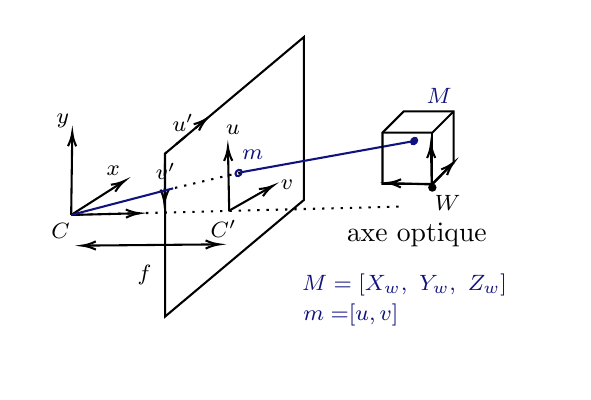
\begin{tikzpicture}[x=0.75pt,y=0.75pt,yscale=-1,xscale=1, scale=0.6]
      
%Shape: Rectangle [id:dp6080383522921334] 
\draw  [line width=0.75]  (261.98,12.03) -- (262.02,142.84) -- (150.52,236.47) -- (150.47,105.66) -- cycle ;
%Shape: Circle [id:dp08023010274775977] 
\draw  [color={rgb, 255:red, 16; green, 18; blue, 125 }  ,draw opacity=1 ][fill={rgb, 255:red, 16; green, 18; blue, 125 }  ,fill opacity=1 ] (350.47,93.07) .. controls (351.83,92.71) and (352.93,93.52) .. (352.93,94.88) .. controls (352.93,96.24) and (351.83,97.64) .. (350.47,98.01) .. controls (349.1,98.37) and (348,97.56) .. (348,96.2) .. controls (348,94.84) and (349.1,93.44) .. (350.47,93.07) -- cycle ;
%Shape: Circle [id:dp3655464346040763] 
\draw  [fill={rgb, 255:red, 0; green, 0; blue, 0 }  ,fill opacity=1 ] (365.12,130.42) .. controls (366.48,130.42) and (367.58,131.52) .. (367.58,132.88) .. controls (367.58,134.25) and (366.48,135.35) .. (365.12,135.35) .. controls (363.75,135.35) and (362.65,134.25) .. (362.65,132.88) .. controls (362.65,131.52) and (363.75,130.42) .. (365.12,130.42) -- cycle ;
%Straight Lines [id:da17745809104725896] 
\draw  [dash pattern={on 4.5pt off 4.5pt}]  (150.02,143.52) -- (150.47,105.66) ;
\draw [shift={(150,145.52)}, rotate = 270.68] [color={rgb, 255:red, 0; green, 0; blue, 0 }  ][line width=0.75]    (10.93,-3.29) .. controls (6.95,-1.4) and (3.31,-0.3) .. (0,0) .. controls (3.31,0.3) and (6.95,1.4) .. (10.93,3.29)   ;
%Straight Lines [id:da05889635157911033] 
\draw  [dash pattern={on 4.5pt off 4.5pt}]  (182.47,78.8) -- (150.47,105.66) ;
\draw [shift={(184,77.52)}, rotate = 139.99] [color={rgb, 255:red, 0; green, 0; blue, 0 }  ][line width=0.75]    (10.93,-3.29) .. controls (6.95,-1.4) and (3.31,-0.3) .. (0,0) .. controls (3.31,0.3) and (6.95,1.4) .. (10.93,3.29)   ;
%Shape: Circle [id:dp5303143417620277] 
\draw  [color={rgb, 255:red, 16; green, 18; blue, 125 }  ,draw opacity=1 ] (209.53,118.71) .. controls (210.9,118.35) and (212,119.15) .. (212,120.52) .. controls (212,121.88) and (210.9,123.28) .. (209.53,123.64) .. controls (208.17,124.01) and (207.07,123.2) .. (207.07,121.84) .. controls (207.07,120.48) and (208.17,119.08) .. (209.53,118.71) -- cycle ;
%Straight Lines [id:da00927428602476521] 
\draw [color={rgb, 255:red, 16; green, 18; blue, 125 }  ,draw opacity=1 ][fill={rgb, 255:red, 16; green, 18; blue, 125 }  ,fill opacity=1 ]   (350.47,95.54) -- (212,120.52) ;
%Straight Lines [id:da32805162479437044] 
\draw    (365.12,130.42) -- (331,129.27) ;
\draw [shift={(329,129.2)}, rotate = 1.93] [color={rgb, 255:red, 0; green, 0; blue, 0 }  ][line width=0.75]    (10.93,-3.29) .. controls (6.95,-1.4) and (3.31,-0.3) .. (0,0) .. controls (3.31,0.3) and (6.95,1.4) .. (10.93,3.29)   ;
%Straight Lines [id:da05612024820893058] 
\draw    (365.12,130.42) -- (380.86,114.19) ;
\draw [shift={(382.25,112.75)}, rotate = 134.12] [color={rgb, 255:red, 0; green, 0; blue, 0 }  ][line width=0.75]    (10.93,-3.29) .. controls (6.95,-1.4) and (3.31,-0.3) .. (0,0) .. controls (3.31,0.3) and (6.95,1.4) .. (10.93,3.29)   ;
%Straight Lines [id:da12713737372353529] 
\draw    (364.65,132.88) -- (364.04,100.2) ;
\draw [shift={(364,98.2)}, rotate = 88.93] [color={rgb, 255:red, 0; green, 0; blue, 0 }  ][line width=0.75]    (10.93,-3.29) .. controls (6.95,-1.4) and (3.31,-0.3) .. (0,0) .. controls (3.31,0.3) and (6.95,1.4) .. (10.93,3.29)   ;
%Shape: Cube [id:dp807415732594561] 
\draw   (325.13,88.8) -- (342.27,71.67) -- (382.25,71.67) -- (382.25,112.75) -- (365.12,129.88) -- (325.13,129.88) -- cycle ; \draw   (382.25,71.67) -- (365.12,88.8) -- (325.13,88.8) ; \draw   (365.12,88.8) -- (365.12,129.88) ;
%Straight Lines [id:da08433615549134643] 
\draw [color={rgb, 255:red, 0; green, 0; blue, 0 }  ,draw opacity=1 ] [dash pattern={on 0.84pt off 2.51pt}]  (338,148.2) -- (75.12,154.88) ;
%Straight Lines [id:da11482119710212657] 
\draw [color={rgb, 255:red, 0; green, 0; blue, 0 }  ,draw opacity=1 ]   (75.12,154.88) -- (75.97,90.75) ;
\draw [shift={(76,88.75)}, rotate = 90.77] [color={rgb, 255:red, 0; green, 0; blue, 0 }  ,draw opacity=1 ][line width=0.75]    (10.93,-3.29) .. controls (6.95,-1.4) and (3.31,-0.3) .. (0,0) .. controls (3.31,0.3) and (6.95,1.4) .. (10.93,3.29)   ;
%Straight Lines [id:da048965394022432385] 
\draw [color={rgb, 255:red, 0; green, 0; blue, 0 }  ,draw opacity=1 ]   (75.12,154.88) -- (116.31,128.59) ;
\draw [shift={(118,127.52)}, rotate = 147.45] [color={rgb, 255:red, 0; green, 0; blue, 0 }  ,draw opacity=1 ][line width=0.75]    (10.93,-3.29) .. controls (6.95,-1.4) and (3.31,-0.3) .. (0,0) .. controls (3.31,0.3) and (6.95,1.4) .. (10.93,3.29)   ;
%Straight Lines [id:da0181640786884405] 
\draw [color={rgb, 255:red, 0; green, 0; blue, 0 }  ,draw opacity=1 ]   (75.12,154.88) -- (128,153.57) ;
\draw [shift={(130,153.52)}, rotate = 178.57] [color={rgb, 255:red, 0; green, 0; blue, 0 }  ,draw opacity=1 ][line width=0.75]    (10.93,-3.29) .. controls (6.95,-1.4) and (3.31,-0.3) .. (0,0) .. controls (3.31,0.3) and (6.95,1.4) .. (10.93,3.29)   ;
%Straight Lines [id:da4676436047615513] 
\draw [color={rgb, 255:red, 16; green, 18; blue, 125 }  ,draw opacity=1 ]   (157,133.52) -- (75.12,154.88) ;
%Straight Lines [id:da7951596067163212] 
\draw [color={rgb, 255:red, 0; green, 0; blue, 0 }  ,draw opacity=1 ]   (86,179.5) -- (192,178.53) ;
\draw [shift={(194,178.52)}, rotate = 179.48] [color={rgb, 255:red, 0; green, 0; blue, 0 }  ,draw opacity=1 ][line width=0.75]    (10.93,-3.29) .. controls (6.95,-1.4) and (3.31,-0.3) .. (0,0) .. controls (3.31,0.3) and (6.95,1.4) .. (10.93,3.29)   ;
\draw [shift={(84,179.52)}, rotate = 359.48] [color={rgb, 255:red, 0; green, 0; blue, 0 }  ,draw opacity=1 ][line width=0.75]    (10.93,-3.29) .. controls (6.95,-1.4) and (3.31,-0.3) .. (0,0) .. controls (3.31,0.3) and (6.95,1.4) .. (10.93,3.29)   ;
%Straight Lines [id:da4782896820641106] 
\draw [color={rgb, 255:red, 0; green, 0; blue, 0 }  ,draw opacity=1 ] [dash pattern={on 0.84pt off 2.51pt}]  (211.07,120.84) -- (157,133.52) ;
%Shape: Rectangle [id:dp446540245188062] 
\draw  [color={rgb, 255:red, 255; green, 255; blue, 255 }  ,draw opacity=1 ] (41.02,5.34) -- (469,5.34) -- (469,280.34) -- (41.02,280.34) -- cycle ;
%Straight Lines [id:da18381069731153055] 
\draw    (202.02,152.01) -- (201.04,102.52) ;
\draw [shift={(201,100.52)}, rotate = 88.86] [color={rgb, 255:red, 0; green, 0; blue, 0 }  ][line width=0.75]    (10.93,-3.29) .. controls (6.95,-1.4) and (3.31,-0.3) .. (0,0) .. controls (3.31,0.3) and (6.95,1.4) .. (10.93,3.29)   ;
%Straight Lines [id:da04744764226882381] 
\draw    (202.56,151.13) -- (235.26,132.51) ;
\draw [shift={(237,131.52)}, rotate = 150.34] [color={rgb, 255:red, 0; green, 0; blue, 0 }  ][line width=0.75]    (10.93,-3.29) .. controls (6.95,-1.4) and (3.31,-0.3) .. (0,0) .. controls (3.31,0.3) and (6.95,1.4) .. (10.93,3.29)   ;

% Text Node
\draw (358,50.9) node [anchor=north west][inner sep=0.75pt]  [font=\footnotesize,color={rgb, 255:red, 16; green, 18; blue, 125 }  ,opacity=1 ]  {$M$};
% Text Node
\draw (364.65,136.28) node [anchor=north west][inner sep=0.75pt]  [font=\footnotesize]  {$W$};
% Text Node
\draw (154,71.9) node [anchor=north west][inner sep=0.75pt]  [font=\footnotesize]  {$u'$};
% Text Node
\draw (129.5,109.4) node [anchor=north west][inner sep=0.75pt]  [font=\footnotesize]  {$ \begin{array}{l}
v'\\
\end{array}$};
% Text Node
\draw (210,99.9) node [anchor=north west][inner sep=0.75pt]  [font=\footnotesize,color={rgb, 255:red, 167; green, 17; blue, 17 }  ,opacity=1 ]  {$\textcolor[rgb]{0.06,0.07,0.49}{m}$};
% Text Node
\draw (294,159) node [anchor=north west][inner sep=0.75pt]   [align=left] {axe optique};
% Text Node
\draw (126,192.9) node [anchor=north west][inner sep=0.75pt]  [font=\footnotesize]  {$f$};
% Text Node
\draw (56.65,159.28) node [anchor=north west][inner sep=0.75pt]  [font=\footnotesize]  {$C$};
% Text Node
\draw (61,70.9) node [anchor=north west][inner sep=0.75pt]  [font=\footnotesize]  {$y$};
% Text Node
\draw (101,112.9) node [anchor=north west][inner sep=0.75pt]  [font=\footnotesize]  {$x$};
% Text Node
\draw (184.65,156.6) node [anchor=north west][inner sep=0.75pt]  [font=\footnotesize]  {$C'$};
% Text Node
\draw (241,123.9) node [anchor=north west][inner sep=0.75pt]  [font=\footnotesize]  {$v$};
% Text Node
\draw (197,79.92) node [anchor=north west][inner sep=0.75pt]  [font=\footnotesize]  {$u$};
% Text Node
\draw (258,199.9) node [anchor=north west][inner sep=0.75pt]  [font=\footnotesize,color={rgb, 255:red, 16; green, 18; blue, 125 }  ,opacity=1 ]  {$M=[ X_{w} ,\ Y_{w} ,\ Z_{w}]$};
% Text Node
\draw (259,223.9) node [anchor=north west][inner sep=0.75pt]  [font=\footnotesize,color={rgb, 255:red, 167; green, 17; blue, 17 }  ,opacity=1 ]  {$\textcolor[rgb]{0.06,0.07,0.49}{m=}\textcolor[rgb]{0.06,0.07,0.49}{[}\textcolor[rgb]{0.06,0.07,0.49}{u,v}\textcolor[rgb]{0.06,0.07,0.49}{]}$};


    \end{tikzpicture}
  \end{overlayarea}
\end{minipage}
\end{frame}


\begin{frame}{Projection d’un point 3D sur le plan image}
  \centering
    $\displaystyle
    \begin{bmatrix}
    u \\ v \\ w
    \end{bmatrix}
    =
    \begin{bmatrix}
    f & 0 & 0 & 0 \\
    0 & f & 0 & 0 \\
    0 & 0 & 1 & 0
    \end{bmatrix}
    \begin{bmatrix}
    R & T \\
    0 & 1
    \end{bmatrix}
    \begin{bmatrix}
    X_w \\ Y_w \\ Z_w \\ 1
    \end{bmatrix}
    $
\end{frame}

%-----------------------------------------------
\begin{frame}
\frametitle{Les différents repères}

\[
\lambda_i 
\begin{pmatrix}
u^{(i)} \\
v^{(i)} \\
1
\end{pmatrix}
=
\begin{pmatrix}
p_{11} & p_{12} & p_{13} & p_{14} \\
p_{21} & p_{22} & p_{23} & p_{24} \\
p_{31} & p_{32} & p_{33} & p_{34}
\end{pmatrix}
\begin{pmatrix}
x_C^{(i)} \\
y_C^{(i)} \\
z_C^{(i)} \\
1
\end{pmatrix}
\]
\end{frame}


\begin{frame}{Modèle de projection — Matrice \( P \)}

\begin{itemize}
  \item<1-> On considère un point 3D \( M = (X, Y, Z) \)
  \item<2-> Il se projette sur un point image \( m = (u, v) \)

  \item<3-> On cherche une relation linéaire homogène :
  \[
  \lambda
  \begin{bmatrix}
  u \cr v \cr 1
  \end{bmatrix}
  P
  =
  \begin{bmatrix}
  X \cr Y \cr Z \cr 1
  \end{bmatrix}
  \]

  \item<4-> \( P \) est une matrice \( 3 \times 4 \), avec 12 inconnues
  \item<5-> En développant les lignes :
  \[
  \lambda u = p_{11}X + p_{12}Y + p_{13}Z + p_{14}
  \]
  \[
  \lambda v = p_{21}X + p_{22}Y + p_{23}Z + p_{24}
  \]
  \[
  \lambda   = p_{31}X + p_{32}Y + p_{33}Z + p_{34}
  \]
\end{itemize}
\end{frame}

%------------------------

\begin{frame}{Équations sans \(\lambda\) et système matriciel}

\begin{itemize}
  \item<1-> Pour un point donné, on élimine \( \lambda \) :
  
  \[
  u (p_{31}X + p_{32}Y + p_{33}Z + p_{34}) = p_{11}X + p_{12}Y + p_{13}Z + p_{14}
  \]
  \[
  v (p_{31}X + p_{32}Y + p_{33}Z + p_{34}) = p_{21}X + p_{22}Y + p_{23}Z + p_{24}
  \]

  \vspace{0.5em}
   \item<2-> Cela donne un système homogène ...
   \[
   \scriptsize
   \begin{cases}
0= & p_{11} x_{C} +p_{12} y_{C}  +p_{13} z_{C} +p_{14} -p_{31} u x_{C} -p_{32} u  z_{C}  -p_{33} u  z_{C}  -p_{34} u \\
0= &  p_{21} x_{C}  +p_{22} y_{C}  +p_{23} z_{C}  +p_{24} -p_{31} v  x_{C}  -p_{32} v  z_{C}  -p_{33} v  z_{C}  -p_{34} v 
\end{cases}
   \]
  \item<3-> En faisant cela pour n points on obtient un système ...
\end{itemize}

\end{frame}

\begin{frame}{Équations sans \(\lambda\) et système matriciel}
  
\[
\resizebox{\textwidth}{!}{$
\left(
\begin{array}{cccccccccccc}
    x_{C}^{(1)} & y_{C}^{(1)} & z_{C}^{(1)} & 1 & 0 & 0 & 0 & 0 & -u^{( 1)} x{C}^{(1)} & -u^{( 1)}y{C}^{(1)} & -u^{( 1)}z_{C}^{(1)} & -u^{(1)}\\
0 & 0 & 0 & 0 & x_{C}^{( 1)} & y_{C}^{( 1)} & z_{C}^{( 1)} & 1 & -v^{( 1)} x_{C}^{( 1)} & -v^{( 1)} y_{C}^{( 1)} & -v^{( 1)} z_{C}^{( 1)} & -v^{( 1)}\\
\vdots  & \vdots  & \vdots  & \vdots  & \vdots  & \vdots  & \vdots  & \vdots  & \vdots  & \vdots  & \vdots  & \vdots \\
x_{C}^{( i)} & y_{C}^{( i)} & z_{C}^{( i)} & 1 & 0 & 0 & 0 & 0 & -u^{( i)} x_{C}^{( i)} & -u^{( i)} y_{C}^{( i)} & -u^{( i)} z_{C}^{( i)} & -u^{( i)}\\
0 & 0 & 0 & 0 & x_{C}^{( i)} & y_{C}^{( i)} & z_{C}^{( i)} & 1 & -v^{( i)} x_{C}^{( i)} & -v^{( i)} y_{C}^{( i)} & -v^{( i)} z_{C}^{( i)} & -v^{( i)}\\
\vdots  & \vdots  & \vdots  & \vdots  & \vdots  & \vdots  & \vdots  & \vdots  & \vdots  & \vdots  & \vdots  & \vdots \\
x_{C}^{( 6)} & y_{C}^{( 6)} & z_{C}^{( 6)} & 1 & 0 & 0 & 0 & 0 & -u^{( 6)} x_{C}^{( 6)} & -u^{( 6)} y_{C}^{( 6)} & -u^{( 6)} z_{C}^{( 6)} & -u^{( 6)}\\
0 & 0 & 0 & 0 & x_{C}^{( 6)} & y_{C}^{( 6)} & z_{C}^{( 6)} & 1 & -v^{( 6)} x_{C}^{( 6)} & -v^{( 6)} y_{C}^{( 6)} & -v^{( 6)} z_{C}^{( 6)} & -v^{( 6)}
\end{array}
\right)
\begin{pmatrix}
p_{11}\\
p_{12}\\
p_{13}\\
p_{14}\\
p_{21}\\
p_{22}\\
p_{23}\\
p_{24}\\
p_{31}\\
p_{32}\\
p_{33}\\
p_{34}
\end{pmatrix} =\begin{pmatrix}
0\\
0\\
0\\
0\\
0\\
0\\
0\\
0\\
0\\
0\\
0\\
0
\end{pmatrix}
$}
\]
\end{frame}

\subsection{En pratiques}

\begin{frame}{Shootin photo : importance de la prise de vue}
  \centering
  \begin{minipage}{0.48\linewidth}
    \centering
    \begin{figure}
      \centering
      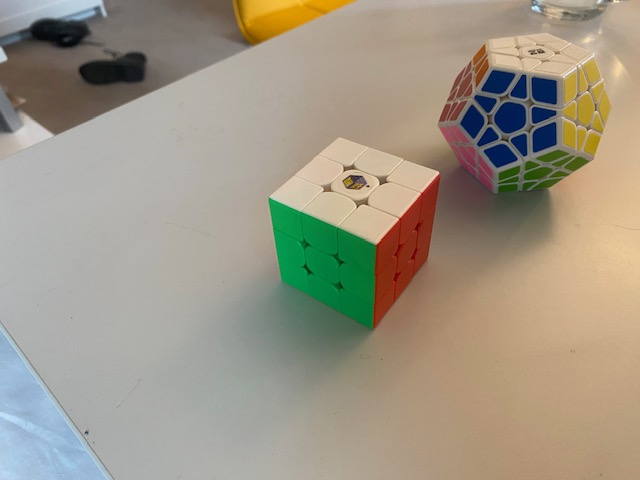
\includegraphics[width=0.48\linewidth]{capture/dodec0.jpg}%
      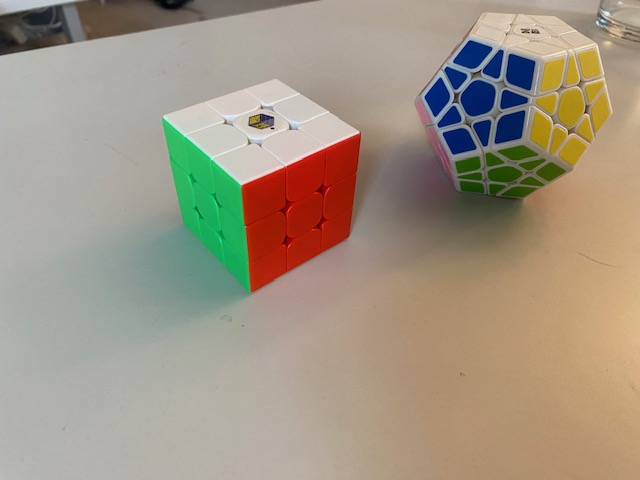
\includegraphics[width=0.48\linewidth]{capture/dodec1.jpg} \\
      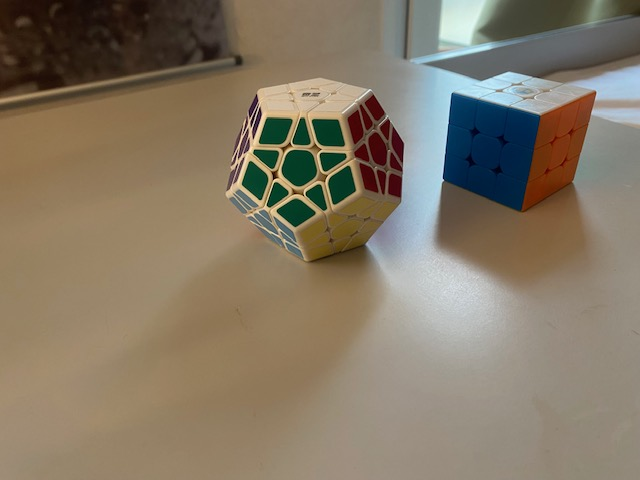
\includegraphics[width=0.48\linewidth]{capture/dodec2.jpg}%
      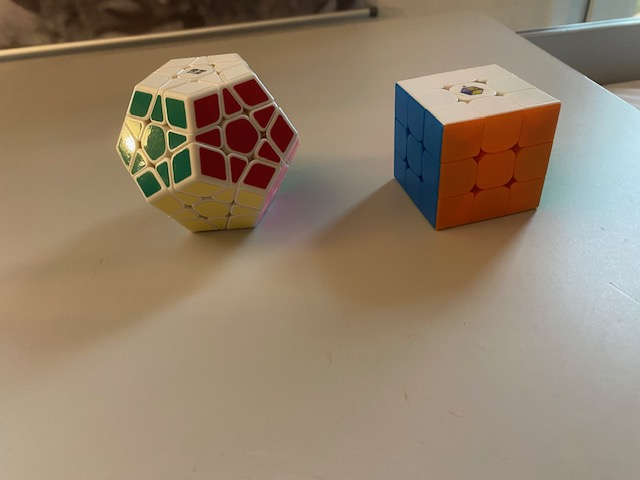
\includegraphics[width=0.48\linewidth]{capture/dodec3.jpg}
      {\footnotesize\textbf{Vues initiales}}
    \end{figure}
  \end{minipage}
  \hfill
  \begin{minipage}{0.48\linewidth}
    \centering
    \begin{figure}
      \centering
      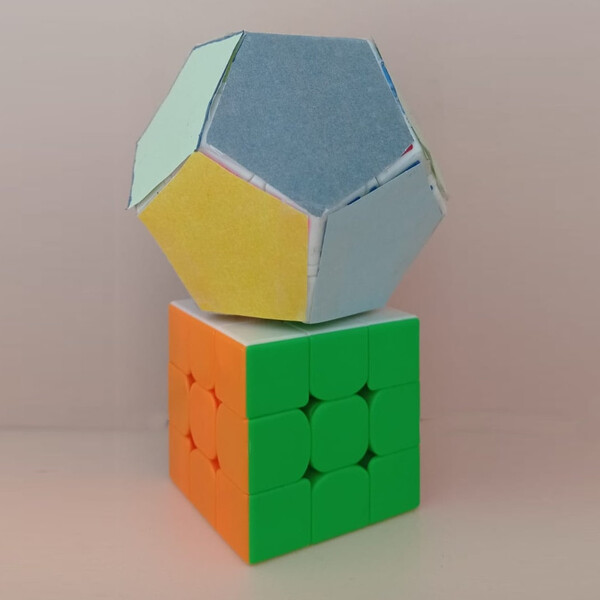
\includegraphics[width=0.48\linewidth]{capture/dodecf0.jpg}%
      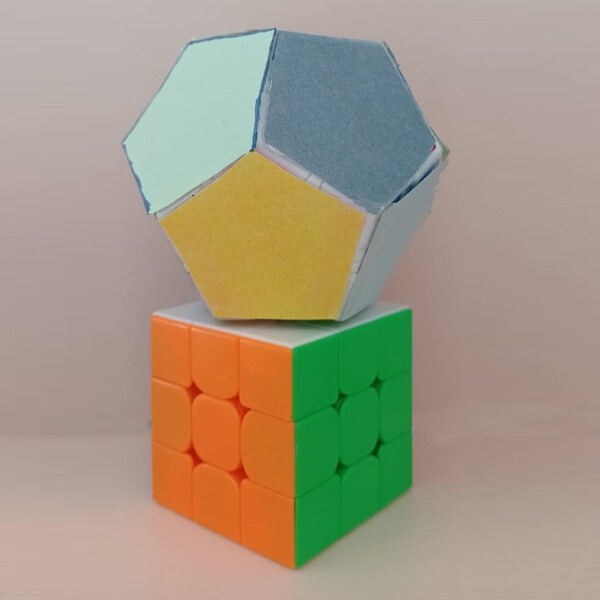
\includegraphics[width=0.48\linewidth]{capture/dodecf1.jpg} \\
      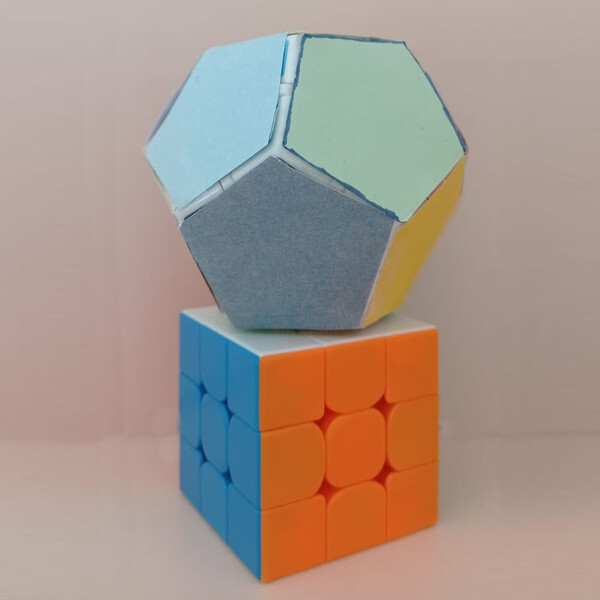
\includegraphics[width=0.48\linewidth]{capture/dodecf2.jpg}%
      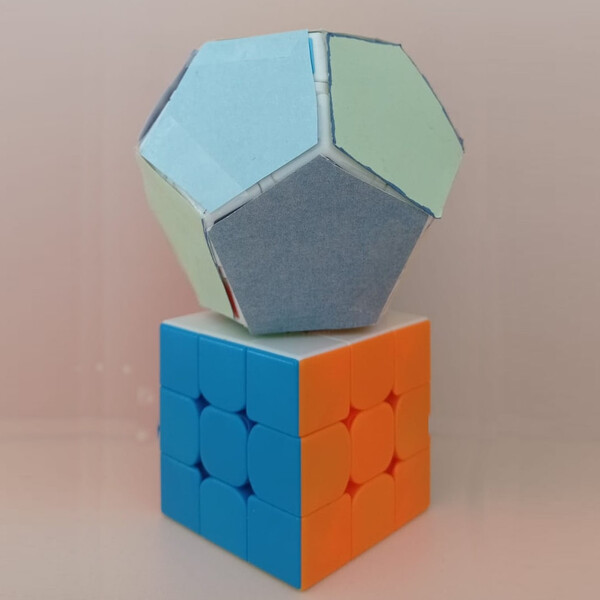
\includegraphics[width=0.48\linewidth]{capture/dodecf3.jpg}
      {\footnotesize\textbf{Vues améliorées}}
    \end{figure}
  \end{minipage}
\end{frame}


\begin{frame}{Calibration}
 \centering
  \begin{minipage}{0.48\linewidth}
    \centering
    \begin{figure}
      \centering
      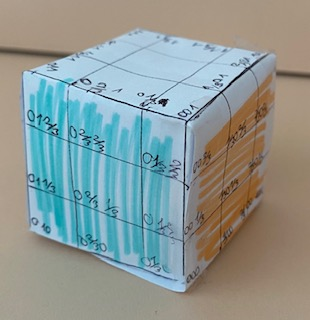
\includegraphics[width=0.7\linewidth]{capture/cube_calibrage.jpg}%
      \caption{Cube calibrage}
    \end{figure}
  \end{minipage}
  \hfill
  \begin{minipage}{0.48\linewidth}
    \centering
    \begin{figure}
      \centering
      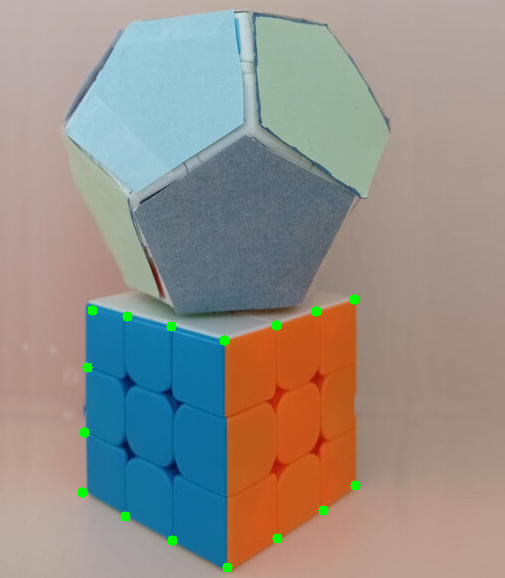
\includegraphics[width=0.8\linewidth]{capture/selection.png}%
      \caption{Selection des points}
    \end{figure}
  \end{minipage}
\end{frame}


